%Every LaTeX file needs a documentclass declaration.
%Possibilities are article, book, letter.  Font size is also declared.

\documentclass[10pt]{article}

%special packages used for symbols, formatting, etc.

\usepackage{amsmath} % contains the align* environment, which is great for manipulating formulas
\usepackage{amssymb} % contains common symbols
\usepackage{amsthm} % has the proof environment
\usepackage[margin=1in]{geometry} % specifies page properties, such as the margin
%\usepackage{siunitx} % useful for typesetting units
\usepackage{xcolor}
\usepackage{graphicx}
% User-defined commands

\newcommand{\newprob}{\medskip \hrule \medskip}
\newcommand{\fanc}[1]{\mathbb{#1}}
\newcommand{\rn}[1]{\fanc{R}^{#1}}
\def\qed{\hspace*{\fill}\rule{1.854mm}{3mm}}  % the fancy box at the end of a proof

%%%%%%%%%%%%%%%%%%%%%%%%%%%%%%%%%%%%%%%%%%%%%%

%beginning of document, every \begin{} also requires an \end{} command.

%\renewcommand{\baselinestretch}{2}

\begin{document}

\pagestyle{empty}  %suppress page numbers, etc.

\begin{center}  %center command, also see flushright, flushleft

{\bf MATH 423-01  Advanced Calculus I

Homework \#3

Assigned: September 14, 2022

Due: September 21, 2022}

\end{center}

\medskip

\hrule   %horizontal line

\bigskip

% list environment: description, itemize, and enumerate

\begin{enumerate}

%%%%%%%%%%%%%%%%%%%%%%

\item  We need to prove that there exists a real number, $x \in \mathbb{R}$, such that $x^2 = 2$.  Consider the set $T = \{t \in \mathbb{R}: t^2 < 2\}$.  Let $x = \sup{(T)}$.  We can prove that $x^2 = 2$ by ruling out the possibilities that $x^2 < 2$ and $x^2 > 2$.

	\begin{enumerate}
	
	\item  ~[Papiernik, J.] Assume to the contrary that $x^2 < 2$.  Prove that this violates the fact that $x$ is an upper bound of $T$.
	
	We want a number in $T$ that is larger than $x$.  We can define $\varepsilon = 2-x^2 > 0$.  We can then find $M \in \mathbb{N}$ such that $\frac{1}{M} < \varepsilon$, by the Archimedean Property.  Note that $\frac{1}{M^2} < \frac{1}{M}$.
	
	Consider the quantity $$\left( x + \frac{1}{M} \right)^2.$$  Figure out what $M$ would need to be so that $\left( x + \frac{1}{M} \right)^2 < 2$.  Argue that $M > 0$.  Prove that $x + \frac{1}{M} \in T$, and finish the proof.

 \begin{proof}
   Consider the set $T = \{t \in \mathbb{R}: t^2 < 2\}$.  Let $x = \sup{(T)}$.  Suppose $x^2 < 2$. Define $\epsilon = 2-x^2 > 0$.  Then by the Archimedean Property, $\exists M \in \mathbb{N}: \frac{1}{M}<\epsilon$.  Therefore $\frac{1}{M^2}<\frac{1}{M}<\epsilon$.  Since $x^2<2$ and $M>0$, then $(x + \frac{1}{M})^2 = x^2+2x*\frac{1}{M}+\frac{1}{M^2}<2$.  Since $(x+\frac{1}{M})^2 < 2$ and $(x+\frac{1}{M}) \in \mathbb{R}$, then $(x+\frac{1}{M}) \in T$.  Therefore x is not an upper bound of $T$.
 \end{proof}
	\item  ~[Powers, S.] Assume to the contrary that $x^2 > 2$.  Prove that this violates the fact that $x$ is the least upper bound of $T$.
	
	We want an upper bound on $T$ that is smaller than $x$.  We can define $\varepsilon = x^2-2 > 0$.  We can then find $N \in \mathbb{N}$ such that $\frac{1}{N} < \varepsilon$, by the Archimedean Property.  Note that $\frac{1}{N^2} > 0$.
	
	Consider the quantity $$\left( x - \frac{1}{N} \right)^2.$$  Figure out what $N$ would need to be so that $\left( x - \frac{1}{N} \right)^2 > 2$.  Argue that $N > 0$.  Prove that $x - \frac{1}{N}$ is a smaller upper bound on $T$, and finish the proof.
 
	 \begin{proof}
     Consider the set $T = \{t \in \mathbb{R}: t^2 < 2\}$.  Let $x = \sup{(T)}$.  Suppose $x^2 > 2$. Define $\epsilon = x^2-2 > 0$. Then by the Archimedean Property, $\exists N \in \mathbb{N}: \frac{1}{N}<\epsilon$. Therefore $\frac{1}{N^2}<\frac{1}{N}<\epsilon$.  Since $x^2>2$ and $N>0$, then $(x - \frac{1}{N})^2 = x^2-2x*\frac{1}{N}+\frac{1}{N^2}>2$.  Since $x = sup(T)$ and $(x-\frac{1}{N})>2$, then $(x-\frac{1}{N})$ is a smaller upper bound of $T$.  Therefore x is not the least upper bound of $T$.  Hence, for the set $T = \{t \in \mathbb{R}: t^2 < 2\}$ with $x = \sup{(T)}$, $\exists x \in \mathbb{R}$ such that $x^2 =2$.
 \end{proof}
	\end{enumerate}
	
%%%%%%%%%%%%%%

\item  ~[Everyone] Decide whether the following statements about suprema and infima are true or false.  Provide a counterexample for any statements that are false.  Provide a proof for any statement that is true.

	\begin{enumerate}
	
	\item  ~[Schipke, K.] A finite, nonempty set always contains its supremum.

\textbf{\textcolor{black}{\underline{Answer:}}}
\textcolor{black}{True.}
	\item  ~[Schipke, K.] If $a < L$ for every element $a$ in the set $A$, then $\sup{(A)} < L$.

\textbf{\textcolor{black}{\underline{Answer:}}}
\textcolor{black}{False}
\begin{proof}
Let $A$ = (0, 1).  Then $a < 1$ for all $a \in A$, but $sup(A) = 1$.  Hence, proving that $sup(A)$ is not less than $L$.
\end{proof}
	\item ~[Schipke, K.] If $A$ and $B$ are sets with the property that $a < b$ for every $a \in A$ and $b \in B$, then it follows that $\sup{(A)} < \inf{(B)}$.
 
\textbf{\textcolor{black}{\underline{Answer:}}}
\textcolor{black}{False}	
\begin{proof}
Let $A = (-1,0)$ and $B = (0,1)$.  Then $a < b$ for all $a \in A$ and $b \in B$, but $sup(A) = 0 = inf(B)$, thus a contradiction to the statement above.
\end{proof}

	\item  ~[Schmidt, S.] If $\sup{(A)} = s$ and $\sup{(B)} = t$, then $\sup{(A+B)} = s+t$, where $$A+B = \{a+b: a \in A \textnormal{ and } b \in B\}.$$
 
 \textbf{\textcolor{black}{\underline{Answer:}}}
\textcolor{black}{True.}
	
	\item  ~[Schmidt, S.] If $\sup{(A)} \leq \sup{(B)}$, then there exists an element $b \in B$ that is an upper bound for $A$.

\textbf{\textcolor{black}{\underline{Answer:}}}
\textcolor{black}{False}
\begin{proof}
Let $A = B = (0,1)$.  Then $sup(A) = sup(B)$, but no element of $B$ is an upper bound for A.
\end{proof}
	\end{enumerate}
	
%%%%%%%%%%%%
	
\item  ~[Staat, E.] The following parts prove that the relation $A \sim B$ is an \emph{equivalence relation}.

	\begin{enumerate}
	
	\item  (Reflexive) Given a set $A$, explain why $A \sim A$.
\begin{proof}
    For any set $A$, the identity mapping $i:A \rightarrow A$ is a bijective mapping.  Therefore, this idea makes $A ~ A$ for all $A$.
\end{proof}
	\item  (Symmetric) Given sets $A$ and $B$, explain why $A \sim B$ is equivalent to stating that $B \sim A$.  Hint: recall that if $f: A \to B$ is injective, then $f^{-1}: B \to A$ exists, and $(f \circ f^{-1})(x) = (f^{-1} \circ f)(x) = x$.
\begin{proof}
    For $A ~ B$ for the given sets $A$ and $B$, then there exists a bijective mapping $f:A\rightarrow B$ and this ensures the existence of the bijective mapping $f^{-1}: B \rightarrow A$, proving that $B ~A$, since the inverse of a bijective mapping again is a bijective mapping.
\end{proof}
	\item  (Transitive) Let $A$, $B$, and $C$ be sets such that $A \sim B$ and $B \sim C$.  Prove that $A \sim C$.  Hint: facts from Homework \#1 will be useful.
 \begin{proof}
     $A ~B$ and $B~C$ for any three sets $A$, $B$, and $C$, then there exists a bijective mapping $f:A\rightarrow B$ and $g: B \rightarrow C$.  This ensures the existence of the bijective mapping $g	\circ f: A \rightarrow C$.  This is true since the composition of two bijective mapping sets is again a bijective mapping.  Therefore $A ~ C$.
 \end{proof}
 \textbf{NOTE:}
 \textcolor{black}{These three properties implies that the tilde $(\sim)$ is an equivalence relation on a universal set $P(x)$ and the set $P(x)$ is partitioned into classes of equipotent sets.  The sets belonging to the same equipotence class are said to have the same potency or the same cardinal number}
	
	\end{enumerate}
	
%%%%%%%%%%%%%

\newpage

\item\label{prob:Cartesian}  ~[Everyone, Delfosse, D.] Let $A$ and $B$ be sets of real numbers.  The \emph{Cartesian product} of $A$ and $B$ is the set $$A \times B = \{(a,b): a \in A \textnormal{ and } b \in B\}.$$  As an example, if $A = \{1,2\}$ and $B = \{x,y,z\}$, then $A \times B = \{(1,x), (1,y), (1,z), (2,x), (2,y), (2,z) \}$.

	\begin{enumerate}
	
	\item  Let $A, B, C, D \subseteq \mathbb{R}$.  If $A \subseteq C$ and $B \subseteq D$, then prove that $A \times B \subseteq C \times D$.
 
\begin{proof}
 Suppose $A=\left\{a,b\right\}$,$B=\left\{p,q\right\}$, $C=\left\{a,b,c\right\}$, and $D=\left\{p,q,r\right\}$.  Then $A \times B=\left\{(a,p),(a,q),(b,p),(b,q)\right\}$ and $C\times D= \left\{(a,p),(a,q),(a,r),(b,p),(b,q),(b,r),(c,p),(c,q),(c,r)\right\}$. Since all the elements of $A \times B$ are also present in $C \times D$, then $A \times B \subseteq \times D$.
 \end{proof}
	\item  The \emph{Cantor pairing function} is defined as $\pi: \mathbb{Z}^{+} \times \mathbb{Z}^{+} \to \mathbb{Z}^{+}$ by $$\pi(m,n) = \frac{1}{2}(m+n)(m+n+1)+n.$$  Write out a table with rows ($m$) and columns ($n$) indexed by $\{0, 1, 2, 3, 4\}$ and compute $\pi(m,n)$ for each entry of the table along the diagonals that go from lower left to upper right.  Use the table to explain who the Cantor pairing function creates a bijection between $\mathbb{Z}^{+} \times \mathbb{Z}^{+}$ and $\mathbb{Z}^{+}$.  This is not proof, but it strongly suggests that the function works.
\par \medskip
 \begin{figure}[!ht]
\centering  %centering can be used to center the image
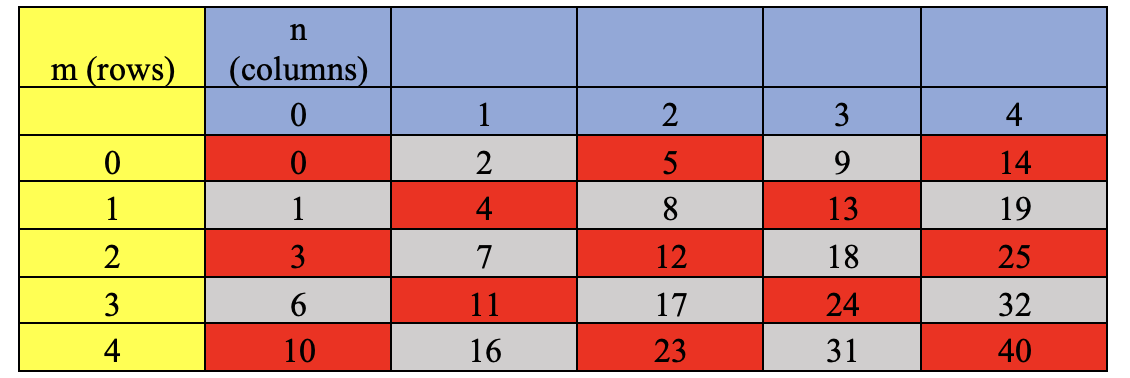
\includegraphics[height=45mm]{Homeworks/Homework 3/AML Homework 3 Graph.png}
 \caption{Graph for Cantor Pairing of $\mathbb{Z}^{+} \times \mathbb{Z}^{+}$ and $\mathbb{Z}^{+}$ }
 \label{f:Chart 1}
\end{figure}	
\textbf{\textcolor{black}{\underline{Answer:}}}
\textcolor{black}{The Cantor pairing function creates a bijection between  $\mathbb{Z}^{+} \times \mathbb{Z}^{+}$ and $\mathbb{Z}^{+}$ is through proving that it is injective and surjective.  We can see in the table that every pair maps to a unique positive integer.  Each pair is mapped to one positive integer only.  So, we can say it is one-one, i.e., injective. We can also observe that all positive integers in the table have an increasing pattern from left to right.  So, for every positive integer, there will be a pair as the preimage.  Hence, the function is surjective.  Since the function is both surjective and injective, then $\mathbb{Z}^{+} \times \mathbb{Z}^{+}$ and $\mathbb{Z}^{+}$ are bijective.}
	\item  Assume that $A$ and $B$ are countable sets.  Prove that $A \times B$ is a countable set.  Hint: use (b).
\begin{proof}
Let $A$ and $B$ be countable sets as stated in the problem.  Then we have that $A = \left\{a_1,a_2,a_3,...\right\}$ and $B = \left\{b_1,b_2,b_3,...\right\}$.  We then have that $A \times B = \left\{(a_i,b_j):a_i  \in A and b_j  \in B\right\}$.  We can define a map from $f:A \times B \rightarrow \mathbb{N}$ such that $f(a_i,b_j)=2^i*3^j$.  We must prove that this function is bijective.
\par \medskip
We first must check whether $f$ is well defined or not, or surjective. Let $(a_i,b_j) = (a_r,b_s)$.  Then $a_i=a_r$ and $b_j=b_s$ i.e., $i=r$ and $j=s$. Now, $f(a_i,b_j )=2^r*3^s$.  Then $f(a_i,b_j )=f(a_r,b_s)$, meaning $f$ is well defined, or surjective.  
\par \medskip
Now to show that f is injective.  Let $f(a_i,b_j )=f(a_r,b_s)$ with $2^i*3^j=2^r*3^s$.  Then $2^{i-r}*3^{j-s}=2^0*3^0$.  Simplifying this down, we get $i-r=0$ and $j-s=0$, meaning $i=r$ and j=s, i.e., $(a_i,b_j )=(a_r,b_s)$.  Considering all of this, then $f$ is injective.

Since $f:A \times B \rightarrow \mathbb{N}$ such that $f$ is injective as $\mathbb{N}$ is countable, then $A \times B$ is countable.  Hence $A \times B = \left\{(a,b): a \in A and b \in B\right\}$ is countable.
\end{proof}
	\item  Let $A_1, A_2, \ldots, A_n$ be a collection of countable sets.  Use induction and (c) to prove that $A_1 \times A_2 \times \cdots \times A_n$ is countable.
 \begin{proof}
By induction, we start with the base case: $n = 2$, which equates to $A_1 \times A_2$, which is countable via part (c).  We then assume it is true for $n = k$, meaning $A_1 \times A_2 \times ... \times A_k$ is countable.  Then we must prove $n = k+1$ is also true, meaning $A_1 \times A_2 \times ... \times A_{k+1}$ is countable.  Writing these elements out, we get that $A_{k+1}=(A_1 \times A_2 \times ... \times A_k)\times A_{k+1}$, with each part being a countable set.  Let $B=A_1 \times A_2 \times ... \times A_k$, which is countable.  Then, $B \times A_{k+1}$ is also countable based on part (c).  Hence $A_1,A_2,...,A_n$ is countable. 
\end{proof}
	
	\end{enumerate}
	
%%%%%%%%%%
	
\item  ~[Wright, A.] Define $$P_n = \{ a_nx^n + a_{n-1}x^{n-1} + \cdots + a_1 x + a_0: a_n, a_{n-1}, \ldots, a_1, a_0 \in \mathbb{Z} \}$$ to be the set of all polynomials of degree $n$ with integer coefficients.

	\begin{enumerate}
	
	\item  Prove that $P_n$ is countable.  Consider the function $f: P_n \to \mathbb{Z}^{n+1}$, where $\mathbb{Z}^{n+1} = \mathbb{Z} \times \mathbb{Z} \times \cdots \times \mathbb{Z}$ with $n+1$ terms, given by $f(p) = (a_n, a_{n-1}, \ldots, a_1, a_0)$.  Show that $f$ is a bijection, and then use Problem \ref{prob:Cartesian}(d).

 \begin{proof}
 Consider the function $f: P_n \rightarrow \mathbb{Z}^{n+1}$ given by $f(P) = (a_n, a_{n-1}, ..., a_1, a_0)$, where $\mathbb{Z}^{n+1} = \mathbb{Z} \times \mathbb{Z} \times ... \times \mathbb{Z}$ $(n+1)$ times and $p(x) = a_nx^n + a_{n-1}x^{n+1} + ... + a_1x + a_0 \in P_n$.  Let $P(x) = a_nx^n + a_{n-1}x^{n-1}+...+a_1x+a0 \in P_n$ and $q(x) = b_nx^n + b_{n-1}x^{n-1}+...+b_1x+b_0 \in P_n$.  Let $f(p(x)) = f(q(x))$, which simplifies to 
 \begin{center}
     $(a_n, a_{n-1},...,a_1, a_0) = (b_n, b_{n-1},...,b_1,b_0)$
     
     $a_n = b_n, a_{n-1} = b_{n-1}, a_{n-2} = b_{n-2},...,a_1 = b_1, a_0 = b_0$
     
     $p(x) = q(x)$
 \end{center}
 This shows that $f:P_n \rightarrow \mathbb{Z}^{n+1}$ by $f(P) = (a_n, a_{n-1},...,a_1, a_0)$ is a one-to one function, or injective.
 \par \medskip
 Now let $(c_n, c_{n-1},...,c_1, c_0) \in \mathbb{Z}^{n+1}$. Choose $P(x) = c_nx^n+c_{n-1}x^{n-1}+...+c_1x+c_0 \in P_n$.  Therefore $f(p(x)) = (c_n, +c_{n-1},...,c_1,c_0)$.  This follows that for any $(c_n, +c_{n-1},...,c_1,c_0) \in \mathbb{Z}^{n+1}$, there exists a preimage under $f$.  So, $f$ is an onto, or surjective, function.  Thus, we get $f:P_n  \rightarrow \mathbb{Z}^{n+1}$ is a bijective mapping.
 \par \medskip
 Since there exists a bijective mapping for $f:P_n  \rightarrow \mathbb{Z}^{n+1}$, then $P_n$ is countable if and only if $\mathbb{Z}^{n+1}$ is also countable.  We know $\mathbb{Z}=$ the set of all integers is a countable set.  Also, we know the Cartesian product of a finite number of countable sets is countable.  Because of these definitions, it can be said that $\mathbb{Z}^{n+1}$ is countable, thus leading to $P_n$ being countable as well.  Hence, $P_n$ is countable.
 \end{proof}
 
	\item  For each $p \in P_n$ define $R(p) = \{x : p(x)=0 \}$ to be the set of roots of $p$.  Prove that $$\bigcup_{p \in P_n} R(p)$$ is countable.
 \begin{proof}
 For each $P \in P_n$,there are almost $n$ zeroes/roots of $P(n)$.  Hence, the number of roots of $P \in P_n$ is finite, i.e., countable.  We know that $P_n$ is countable.  We also know that "Every countable union of countable sets is countable."  Therefore, $$\bigcup_{p \in P_n} R(p)$$ is countable since $P_n$ is countable and $R(P)$ is countable for each $P \in P_n$.  Hence $$\bigcup_{p \in P_n} R(p)$$ is countable.
 \end{proof}	
 
	\item  An \emph{algebraic number} is any number that is a root of a polynomial equation $p(x)=0$, where the coefficients of $p$ are integers.  Prove that the set of algebraic numbers is countable.
 \begin{proof}
     Consider the polynomial $p(x)$ with integer coefficients.  Then the polynomial is of the form $p(x)=a_0 +a_1x+...+a_n*x^n$ where $a_i's$ are integers.  Hence, it is clear that the set of all integer polynomials is isomorphic to $Z^{n+1}$.  Since the function $f$ is defined as $p(x) 	\mapsto (a_0, a_1,...,a_n)$ is an isomorphism.  Note that the set of all integers is countable.  Then $Z^{n+1}$ is countable.  Also, a polynomial of degree $n$ has exactly $n$ roots.  The set of all roots of integer polynomial now becomes the union of countable sets.  Observe that countable union of countable sets is countable. Hence, the roots of the integer polynomial are countable. Therefore, the set of all algebraic numbers is countable.
 \end{proof}
	
	\end{enumerate}
	
%%%%%%%%%%%%

\newpage
	
\item\label{prob:Cantor}  ~[Smith, G.] This problem outlines a proof that the interval $(0,1)$ is uncountable.

	Assume to the contrary that $(0,1)$ is countable.  This means that there exists a bijection $f: \mathbb{N} \to (0,1)$.  Thus for $m \in \mathbb{N}$ we have $f(m) \in (0,1)$, and we can write $f(m) = 0.a_{m1}a_{m2}a_{m3}a_{m4}\ldots$, where $a_{mn} \in \{0, 1, 2, \ldots, 9\}$.  This means that $f(m)$ is the decimal expansion of $f(m)$.  We can then list out all of the elements of $(0,1)$ using the table below.
		$$\begin{array}{ccccccccc}
		\mathbb{N} & & (0,1) & & & & & & \\\hline
		1 & \longleftrightarrow & f(1) & = & 0.\mathbf{a_{11}} & a_{12} & a_{13} & a_{14} & \cdots\\
		2 & \longleftrightarrow & f(2) & = & 0.a_{21} & \mathbf{a_{22}} & a_{23} & a_{24} & \cdots\\
		3 & \longleftrightarrow & f(3) & = & 0.a_{31} & a_{32} & \mathbf{a_{33}} & a_{34} & \cdots\\
		4 & \longleftrightarrow & f(4) & = & 0.a_{41} & a_{42} & a_{43} & \mathbf{a_{44}} & \cdots\\
		& &  \vdots & & & & & & \ddots\\
		\end{array}$$
	Since $(0,1)$ is assumed to be countable, this table contains every number in $(0,1)$.
	
	Define a real number $x \in (0,1)$ with the decimal expansion $x = 0.b_{1}b_{2}b_{3}b_{4}\ldots$, where
		$$b_n = \left\{\begin{array}{c@{\textnormal{ if }}l}
		2 & a_{nn} \neq 2\\
		3 & a_{nn} = 2.\\
		\end{array}\right.$$
		
	\begin{enumerate}
	
	\item  Explain why $x$ cannot be $f(1)$.
 
	\textbf{\underline{Answer:}}
 \textcolor{black}{Here $x = 0*b_1b_2b_3b_4...$ where 
 \begin{equation}
  b_n=% 
  \begin{cases}
    2, if,  a_{nn} \neq 2 \\
    3, if,  a_{nn}=2.
  \end{cases}
\end{equation}
Therefore, $b_1 = 2$ if $a_{11} \neq 2$ or $b_n = 3$ if $a_{11} = 2$.  Hence $b_1 \neq a_{11}$.  So $x = 0*b_1b_2b_3b_4...$ and $f(1) = 0*a_{11}a_{12}a_{13}...$ are not equal, meaning $x$ can not be $f(1)$.
}
 
	\item  Explain why $x$ cannot be $f(2)$, and in general why $x \neq f(m)$, for every $m \in \mathbb{N}$.
 
	\textbf{\underline{Answer:}}
 \textcolor{black}{Given
 \begin{equation}
  b_n=% 
  \begin{cases}
    2, if,  a_{nn} \neq 2 \\
    3, if,  a_{nn}=2.
  \end{cases}
\end{equation}
$b_2 = 2$ if $a_{22} \neq 2$ or $b_2 = 3$ if $a_{22} = 2$, so $b_2 \neq a_{22}$.  Hence $0*b_1b_2b_3... \neq 0*a_{21}a_{22}a_{23}...$.  Therefore, $x$ cannot be $f(2)$.  In general, for any $m \in \mathbb{N}$, $b_m \neq a_{mm}$.  Which means $0*b_1b_2...b_mb_{m+1}... \neq 0*a_{m1}a_{m2}...a_{mm}...$, $b_m$ and $a_{mm}$ are different which leads to $x \neq f(m), \forall m \in \mathbb{N}$.
}
 
	\item  Identify a contradiction and prove that $(0,1)$ is uncountable.
 
	\textbf{\underline{Answer:}}
 \textcolor{black}{Here we get $x = 0*b_1b_2b_3b_4...$ where 
 \begin{equation}
  b_n=% 
  \begin{cases}
    2, if,  a_{nn} \neq 2 \\
    3, if,  a_{nn}=2.
  \end{cases}
\end{equation}
Such that $x \in (0,1)$ but $x \neq f(m)$ for any $m \in \mathbb{N}$, which is a contradiction to the fact that $f$ is bijective from $\mathbb{N}$ to $(0,1)$.
}

\textcolor{black}{For $x = 0*b_1b_2b_3b_4...$ where 
 \begin{equation}
  b_n=% 
  \begin{cases}
    a, if,  a_{nn} \neq a \\
    b, if,  a_{nn}=a.
  \end{cases}
\end{equation}
, with $a \neq b$.  For any $a,b \in \mathbb{R}$, we get uncountable points in $(0,1)$.  So $(0,1)$ is uncountable.
}
 
	\end{enumerate}
	
%%%%%%%%
	
\item  ~[Aitchison, A.] Let $S$ be the set of all sequences of $0$s and $1$s, or $$S = \{(a_1, a_2, a_3, \ldots) : a_n = 0 \textnormal{ or } 1 \}.$$  Use an argument similar to the one in Problem \ref{prob:Cantor} to show that $S$ is uncountable.
\begin{proof}
    Let $S$ be countable.  Then there exists a bijection $f: \mathbb{N} \rightarrow S$, so $\forall m \in \mathbb{N}$, $f(m) \in S$, i.e., $f(m) = (a_{m1}, a_{m2}, a_{m3},...)$ where $\forall n \in \mathbb{N}, a_{mn} = 0$ or $1, \forall m \in \mathbb{N}$.  Since $f$ is a bijection, then the total list of all elements in $S$ can be given as:
    \begin{center}
        $f(1) = (a_{11}, a_{12}, a_{13},...)$
        
        $f(2) = (a_{21}, a_{22}, a_{23},...)$
        
        $...$
        
        $f(m) = (a_{m1}, a_{m2}, a_{m3},...)$
        
        $...$
        
        $a_{mn} = 0$ on 0 or 1, $\forall m \in \mathbb{N}, \forall n \in \mathbb{N}$
    \end{center}
    Define $x = (b_1, b_2, b_3,...)$, where 
\begin{equation}
  b_m=% 
  \begin{cases}
    0, if,  a_{mm} = 1 \\
    1, if,  a_{mm}=0.
  \end{cases}
\end{equation}
Therefore $x \in S$, hence $b_m = 0$ or $1, \forall m \in \mathbb{N}$.  Now the mth term of $x$ is different from the mth term of $f(m), \forall m \in \mathbb{N}$.  Therefore $x \neq f(m), \forall m \in \mathbb{N}$.  This is a contradiction as $x \in S$.  Therefore S is uncountable.
\end{proof}
\end{enumerate}

\end{document}
